% Options for packages loaded elsewhere
\PassOptionsToPackage{unicode}{hyperref}
\PassOptionsToPackage{hyphens}{url}
\PassOptionsToPackage{dvipsnames,svgnames,x11names}{xcolor}
\documentclass[
  11pt,
]{ctexart}
\usepackage{xcolor}
\usepackage[margin=2.5cm]{geometry}
\usepackage{amsmath,amssymb}
\setcounter{secnumdepth}{-\maxdimen} % remove section numbering
\usepackage{iftex}
\ifPDFTeX
  \usepackage[T1]{fontenc}
  \usepackage[utf8]{inputenc}
  \usepackage{textcomp} % provide euro and other symbols
\else % if luatex or xetex
  \usepackage{unicode-math} % this also loads fontspec
  \defaultfontfeatures{Scale=MatchLowercase}
  \defaultfontfeatures[\rmfamily]{Ligatures=TeX,Scale=1}
\fi
\usepackage{lmodern}
\ifPDFTeX\else
  % xetex/luatex font selection
\fi
% Use upquote if available, for straight quotes in verbatim environments
\IfFileExists{upquote.sty}{\usepackage{upquote}}{}
\IfFileExists{microtype.sty}{% use microtype if available
  \usepackage[]{microtype}
  \UseMicrotypeSet[protrusion]{basicmath} % disable protrusion for tt fonts
}{}
\makeatletter
\@ifundefined{KOMAClassName}{% if non-KOMA class
  \IfFileExists{parskip.sty}{%
    \usepackage{parskip}
  }{% else
    \setlength{\parindent}{0pt}
    \setlength{\parskip}{6pt plus 2pt minus 1pt}}
}{% if KOMA class
  \KOMAoptions{parskip=half}}
\makeatother
\usepackage{graphicx}
\makeatletter
\newsavebox\pandoc@box
\newcommand*\pandocbounded[1]{% scales image to fit in text height/width
  \sbox\pandoc@box{#1}%
  \Gscale@div\@tempa{\textheight}{\dimexpr\ht\pandoc@box+\dp\pandoc@box\relax}%
  \Gscale@div\@tempb{\linewidth}{\wd\pandoc@box}%
  \ifdim\@tempb\p@<\@tempa\p@\let\@tempa\@tempb\fi% select the smaller of both
  \ifdim\@tempa\p@<\p@\scalebox{\@tempa}{\usebox\pandoc@box}%
  \else\usebox{\pandoc@box}%
  \fi%
}
% Set default figure placement to htbp
\def\fps@figure{htbp}
\makeatother
\setlength{\emergencystretch}{3em} % prevent overfull lines
\providecommand{\tightlist}{%
  \setlength{\itemsep}{0pt}\setlength{\parskip}{0pt}}
\usepackage{bookmark}
\IfFileExists{xurl.sty}{\usepackage{xurl}}{} % add URL line breaks if available
\urlstyle{same}
\hypersetup{
  colorlinks=true,
  linkcolor={Maroon},
  filecolor={Maroon},
  citecolor={Blue},
  urlcolor={Blue},
  pdfcreator={LaTeX via pandoc}}

\author{}
\date{}

\begin{document}

\section{公开强震动数据约束下早期 P
波预测地震动的可预测性边界}\label{ux516cux5f00ux5f3aux9707ux52a8ux6570ux636eux7ea6ux675fux4e0bux65e9ux671f-p-ux6ce2ux9884ux6d4bux5730ux9707ux52a8ux7684ux53efux9884ux6d4bux6027ux8fb9ux754c}

周浩宇\(^{1}\)，马强\(^{1,*}\)

\(^{1}\) 中国地震局工程力学研究所，哈尔滨 150080

*通讯作者：马强，maqiang@iem.ac.cn。作者邮箱：zhouhaoyiu@gmail.com。ORCID：周浩宇，0009-0003-8817-1209；马强，0000-0002-9768-5223。

\textbf{基金项目}：无。

\subsection{摘要}\label{ux6458ux8981}

地震预警需要在强震动充分到达前，根据最早观测到的 P
波估计后续地震动强度。早期 P
波能提供多少强震动信息，以及这些信息在跨区域使用时何时失效，仍缺少以公开强震动数据为基础的统一检验。本文构建事件-台站级公开基准，以
P 到时后 1、2、3、5 和 10 s 波形窗口预测 PGA、PGV
和反应谱加速度，主证据来自 InstanceGM 和本地转换的 K-NET，外部检验来自
AQ2009GM、CWA 官方 PGA/PGV 数据层和欧洲强震动记录。统一清单包含
2,460,425 条记录；AQ2009GM 流式处理得到 345,226 条有效 PGA/PGV 样本；CWA
2011 年公开 benchmark 得到 5,882 条官方 PGA/PGV 样本。结果表明，加入早期
P 波特征后，held-station 测试中的强震动预测误差稳定降低，10 s 窗口下
InstanceGM PGA、InstanceGM PGV 和 K-NET PGA 的 MAE 分别降低
35.5\%、52.6\% 和 49.9\%。强震动尾部、bootstrap、source-path
support、AQ2009GM、CWA 和 ESM 检验均保留同一信息增益。跨区域 transfer
显示清晰边界：source-domain conformal 区间在目标区明显欠覆盖，50--100
条目标区校准样本可使覆盖率接近 0.90，但区间宽度显著增大。本文给出早期 P
波窗口长度、强震动尾部漏报风险和跨区域不确定性之间的可测量关系，为公开数据约束下的地震预警模型评估提供基准。

\textbf{关键词}：地震预警；早期 P
波；强震动预测；跨区域迁移；不确定性；公开基准

\subsection{0 引言}\label{ux5f15ux8a00}

地震预警的核心任务是在破坏性地震动尚未充分到达前，对目标台站可能经历的强震动作出估计。P
波到时后的最初几秒是单台站最早可获得的波形证据，其中包含震源破裂初始发展、传播路径、场地响应和仪器记录条件共同作用后的观测信息。预警评估需要从随机测试集平均误差推进到可部署场景：早期信息在未见事件、未见台站和不同区域中能稳定贡献多少预测能力。

已有研究从 P
波幅值、特征周期、震级快速估计、台站网络触发和机器学习模型等角度发展了多种地震预警方法。近年来，深度学习和大规模公开数据提高了相位拾取、事件检测和地震动估计的可用性，也让跨数据集验证成为可能。与此同时，强震动预测的高后果错误通常发生在分布尾部和区域迁移场景中。一个模型可以降低平均误差，同时仍然对最强地震动低估，或者把源区域的残差分布错误地用于目标区域。

本文把``早期 P 波是否有用''进一步拆成三个可检验问题。第一，早期 P
波在严格 held-out 事件和台站条件下，是否提供 source-path metadata
之外的信息。第二，这种信息在强震动尾部、pre-peak
记录和重采样检验中是否仍然存在。第三，在跨区域 transfer
中，源区域模型和不确定性估计何时失效，目标区域需要多少校准样本才能恢复覆盖率。

公开强震动数据为上述问题提供了样本基础，也带来溯源约束。不同数据集的分量方向、加速度单位、P
到时定义、台站场地信息和 PGA/PGV/SA
目标变量并不一致。若不把这些差异写入数据链路，模型可能把单位、网络或标注差异学习成区域物理信号。本文以事件-台站记录为基本样本，将短
P
波窗口、预警时可获得的元数据和同一台站后续观测到的强震动目标连接起来，并把每一层证据限定在其实际支持的结论范围内。

本文的目标是估计离线信息边界。实时通信延迟、触发策略、报警阈值和公众响应属于工程系统层面，不在本文主证据范围内。本文关注的是在给定
P 到时和事件-台站记录后，早期 P 波能否减少后续 PGA、PGV 或 SA
的预测误差，以及这种减少能否跨区域转移。

\subsection{1 数据与方法}\label{ux6570ux636eux4e0eux65b9ux6cd5}

\subsubsection{1.1
公开数据源与证据角色}\label{ux516cux5f00ux6570ux636eux6e90ux4e0eux8bc1ux636eux89d2ux8272}

主基准使用 InstanceGM 和 K-NET。InstanceGM
提供大规模地震动目标和多样的震源-路径覆盖，是多目标 PGA、PGV 和 SA
检验的主数据源。K-NET 提供日本强震动记录，本文将原始 BSON 包本地转换为
HDF5 波形和 CSV 元数据，分量统一为 Z、N、E，其中 UD 映射为 Z，NS 映射为
N，EW 映射为 E。K-NET 加速度按 gal 处理，即 cm/s\^{}2。转换过程保留在
provenance 中。

外部证据层承担不同任务。AQ2009GM 用于独立 SeisBench 强震动检验；本文采用
chunk-streaming 方式处理全部本地 manifest chunk，提取早窗特征、PGA/PGV
和事件-台站标识，保存小特征表后删除原始 chunk。CWA 作为官方 PGA/PGV
数据层，当前仅处理公开 benchmark 的 2011 年样本，不写成完整 2011--2021
年验证。ESM 用于欧洲强震动外部域和区域 GMM screening；本地 ESM
头段缺少显式 P 到时，本文采用理论 P 到时并进行 Vp 敏感性和 envelope
onset spot audit。STEAD 和 Iquique
用于相位拾取迁移审计，PNWAccelerometers 仅作为波形峰值幅度稳健性检查。

统一 manifest 当前包含 2,460,425 条记录。InstanceGM 贡献 1,159,223
条地震动记录；K-NET 贡献 22,119 条完整 ZNE 强震动记录。AQ2009GM
流式处理后保留 345,226 条有效 PGA/PGV 特征记录，涉及 60,310 个事件和 66
个台站。CWA 2011 年层保留 5,882 条有效记录，涉及 775 个事件和 705
个台站。ESM 本地包得到 134,250 个早窗特征行，涉及 861 个事件和 1,568
个台站。

\begin{figure}
\centering
\pandocbounded{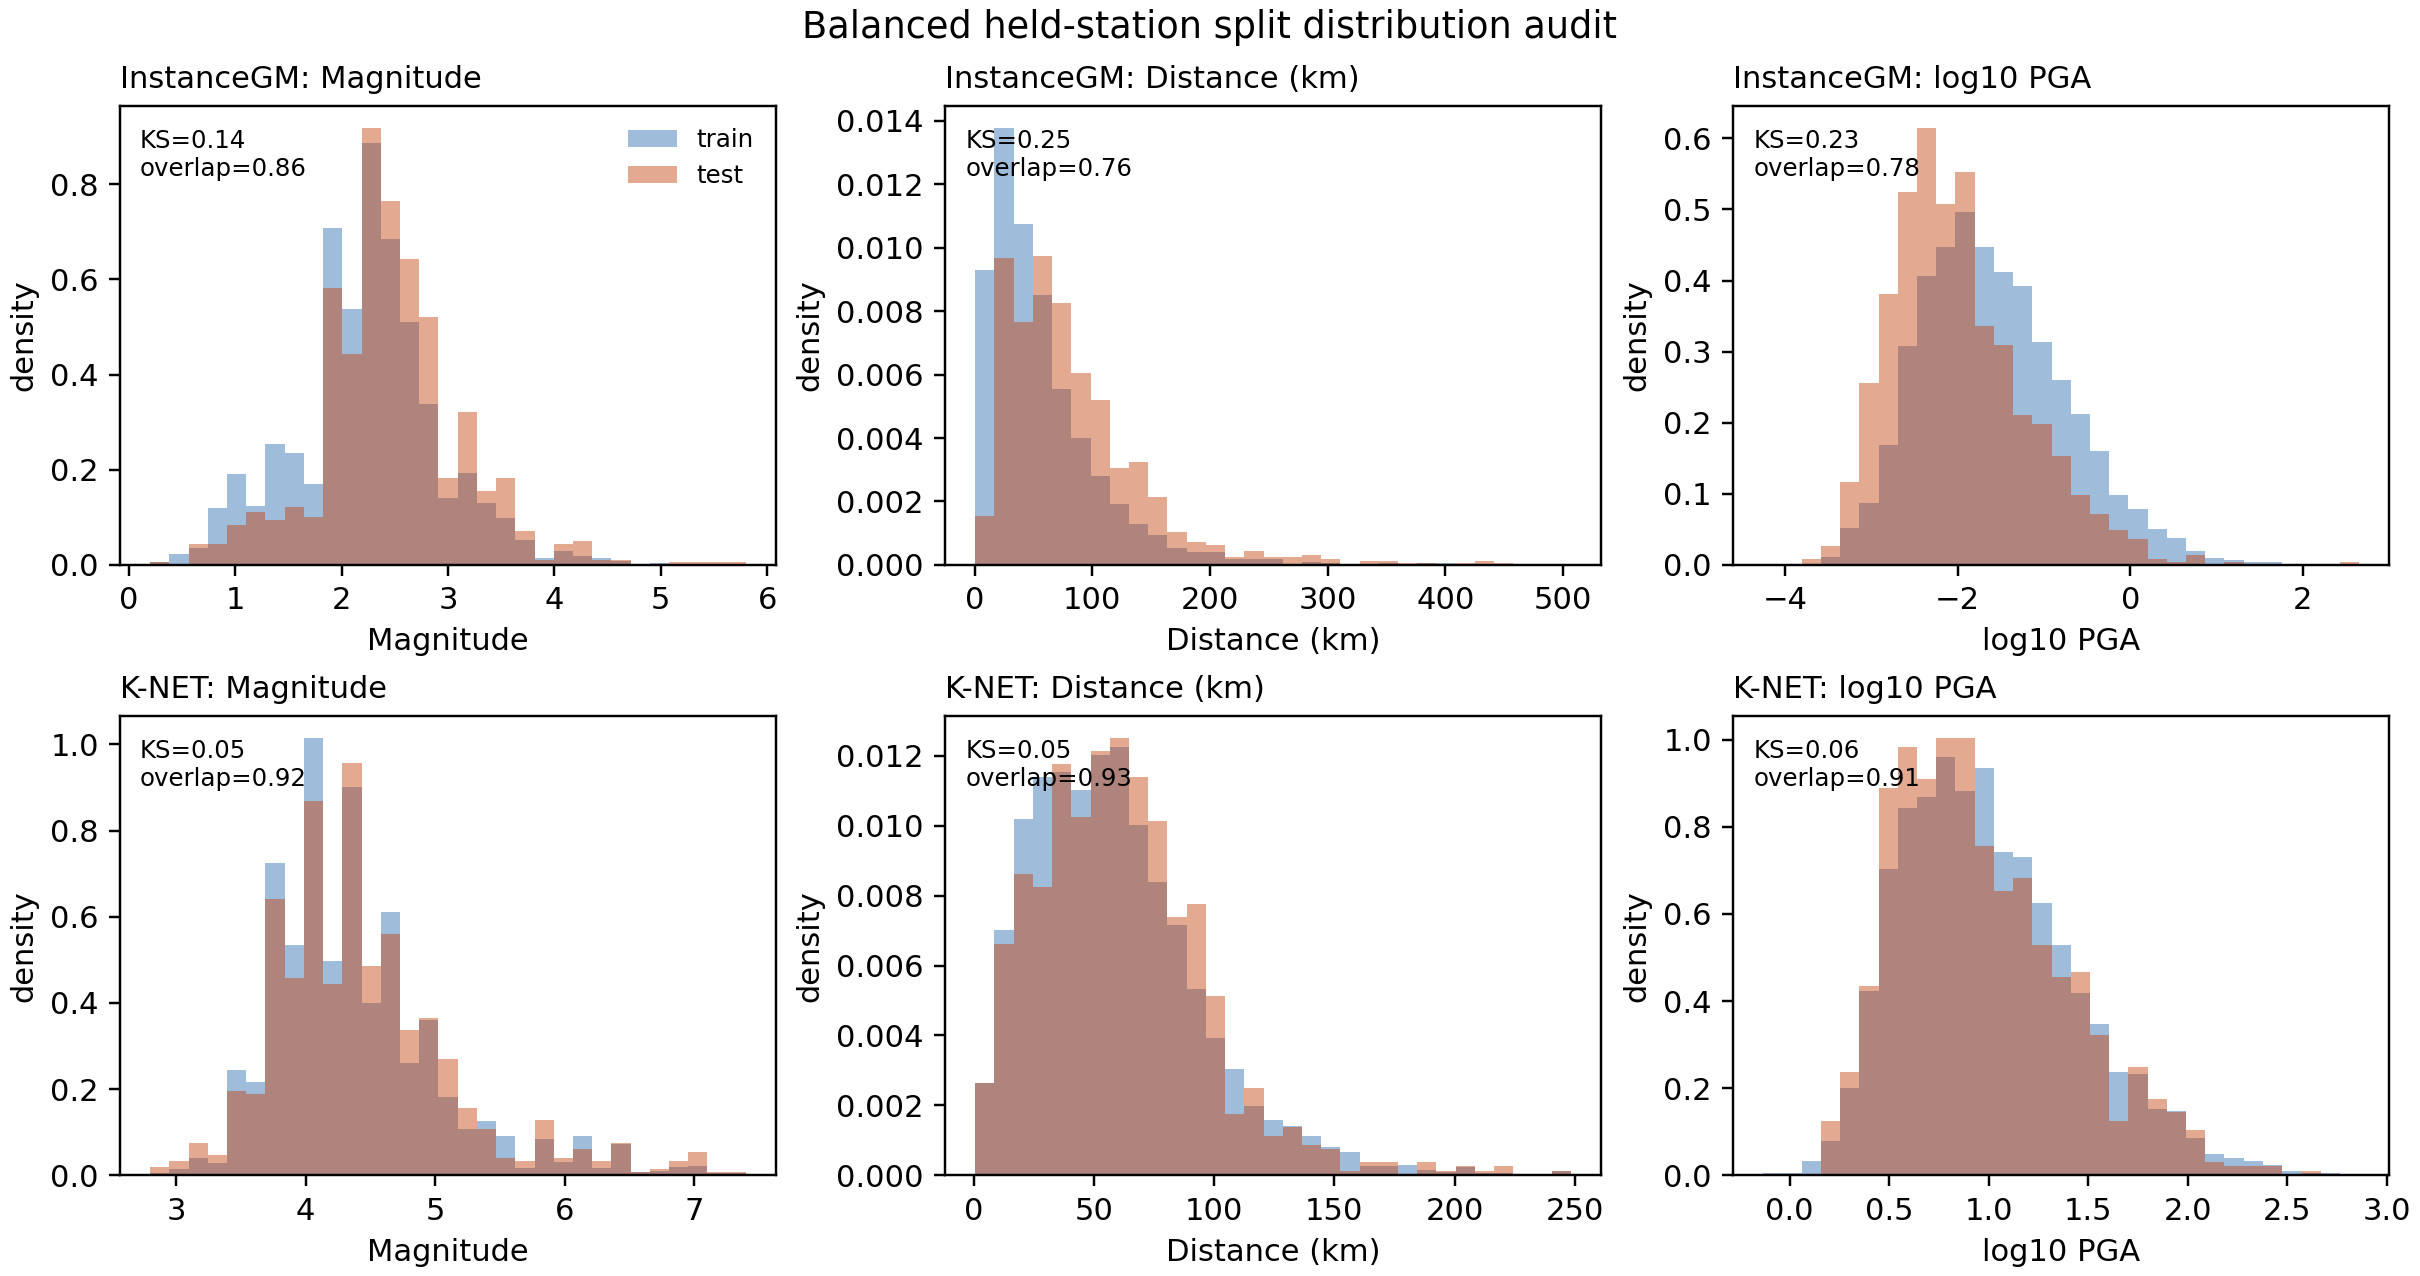
\includegraphics[keepaspectratio,alt={数据层和任务覆盖。InstanceGM 与 K-NET 构成主强震动检验，AQ2009GM、CWA 和 ESM 提供外部证据层；不同数据源只在其目标变量和标注条件允许的范围内使用。 Fig. 1 Dataset layers and task coverage.}]{figures/ground_motion_audit/balanced_station_distribution_audit_panel.png}}
\caption{数据层和任务覆盖。InstanceGM 与 K-NET
构成主强震动检验，AQ2009GM、CWA 和 ESM
提供外部证据层；不同数据源只在其目标变量和标注条件允许的范围内使用。
Fig. 1 Dataset layers and task coverage.}
\end{figure}

\subsubsection{1.2
事件-台站样本、早窗特征与目标变量}\label{ux4e8bux4ef6-ux53f0ux7ad9ux6837ux672cux65e9ux7a97ux7279ux5f81ux4e0eux76eeux6807ux53d8ux91cf}

每条样本对应一个事件在一个台站的一条记录。以 P 到时为起点，提取
1、2、3、5 和 10 s
早期窗口。波形特征包括三分量最大绝对值、RMS、标准差、95
分位绝对幅值、水平向最大值、三分量向量最大值和向量
RMS。全记录峰值不进入预测特征，避免目标泄漏。目标变量在 log10
单位下建模，包括 PGA、PGV 和可用的反应谱加速度 SA(0.3 s)、SA(1.0
s)、SA(3.0 s)。

输入信息分为四组：source-path metadata；早期 P 波特征；metadata 加早期 P
波；跨区域 transfer 中只使用早期 P 波统计。metadata
包括震级、深度、距离和可用场地信息。跨区域 transfer
排除震级、距离、场地、event id 和 station
id，目的在于单独检验早期波形统计本身的可迁移性。

\subsubsection{1.3
划分、模型和评价指标}\label{ux5212ux5206ux6a21ux578bux548cux8bc4ux4ef7ux6307ux6807}

本文使用 held-event 和 held-station 划分。held-event
保证训练集和测试集事件不重叠，held-station
保证训练集和测试集台站不重叠。所有主表均检查 group overlap，主验证中
overlap 为 0。held-station
是本文更重视的泛化场景，因为预警模型部署时常面对训练集中未出现的目标台站。

主模型采用稳定的树模型和保守超参数。本文固定模型族，把比较重点放在相同
split 和目标定义下早期 P 波是否相对 metadata-only
基线降低误差。评价指标为 log10 目标单位下的
MAE、RMSE、\(R^2\)、强震动尾部 MAE 和相对误差降低率。相对降低率定义为

\[
100 \times \frac{\mathrm{MAE}_{\mathrm{baseline}}-\mathrm{MAE}_{\mathrm{waveform}}}{\mathrm{MAE}_{\mathrm{baseline}}}.
\]

不确定性使用 conformal interval
评估。域内测试采用目标域校准残差。跨区域测试分别使用 source-domain
conformal、target-offset calibration 和 target-domain
conformal，以区分源域残差、目标区偏移和目标区残差宽度的作用。校准样本量审计固定源域模型，只从目标区抽取
10、25、50、100、250 和 1000 条记录估计一个 offset 和 conformal
残差宽度。

\subsubsection{1.4 补充审计}\label{ux8865ux5145ux5ba1ux8ba1}

bootstrap 审计对 held-station
测试记录成对重采样，估计相对误差降低率的置信区间。source-path support
审计只根据震级和距离将测试记录限制在训练集中心支持范围内，不使用目标幅值筛选。强震动尾部审计聚焦目标幅值最高
5\% 的记录。pre-peak 审计从 K-NET PGA 中剔除早窗水平峰值已接近最终 PGA
的记录，用于检验短窗结果是否仍有 lead-time 含义。轻量 CNN
波形编码器用于模型复杂度对照，不能作为 foundation model 结果。

\subsection{2 结果}\label{ux7ed3ux679c}

\subsubsection{2.1 早期 P
波在未见台站上提供稳定信息增益}\label{ux65e9ux671f-p-ux6ce2ux5728ux672aux89c1ux53f0ux7ad9ux4e0aux63d0ux4f9bux7a33ux5b9aux4fe1ux606fux589eux76ca}

在主 held-station 测试中，加入早期 P
波特征后，多个目标的预测误差稳定降低。10 s 窗口下，metadata
加早期波形模型相对 metadata-only 基线的 MAE 降低率为：InstanceGM PGA
35.5\%、InstanceGM PGV 52.6\%、InstanceGM SA03 26.0\%、SA10 20.9\%、SA30
27.8\%、K-NET PGA
49.9\%。这些测试排除了训练和测试台站重叠，说明增益不依赖同一台站重复出现。

信息增益随 P 窗口长度增加而变化。K-NET PGA 的 held-station 误差降低率从
1 s 的 11.3\% 增至 5 s 的 23.3\%，10 s 达到 49.9\%。InstanceGM PGV 在 1
s 已有 40.1\% 降低，5 s 为 45.4\%，10 s 为
52.6\%。这表明不同强震动目标的早期可观测性不同：PGV
对早期幅值和能量特征更敏感，PGA 对窗口长度的依赖更强。

\begin{figure}
\centering
\pandocbounded{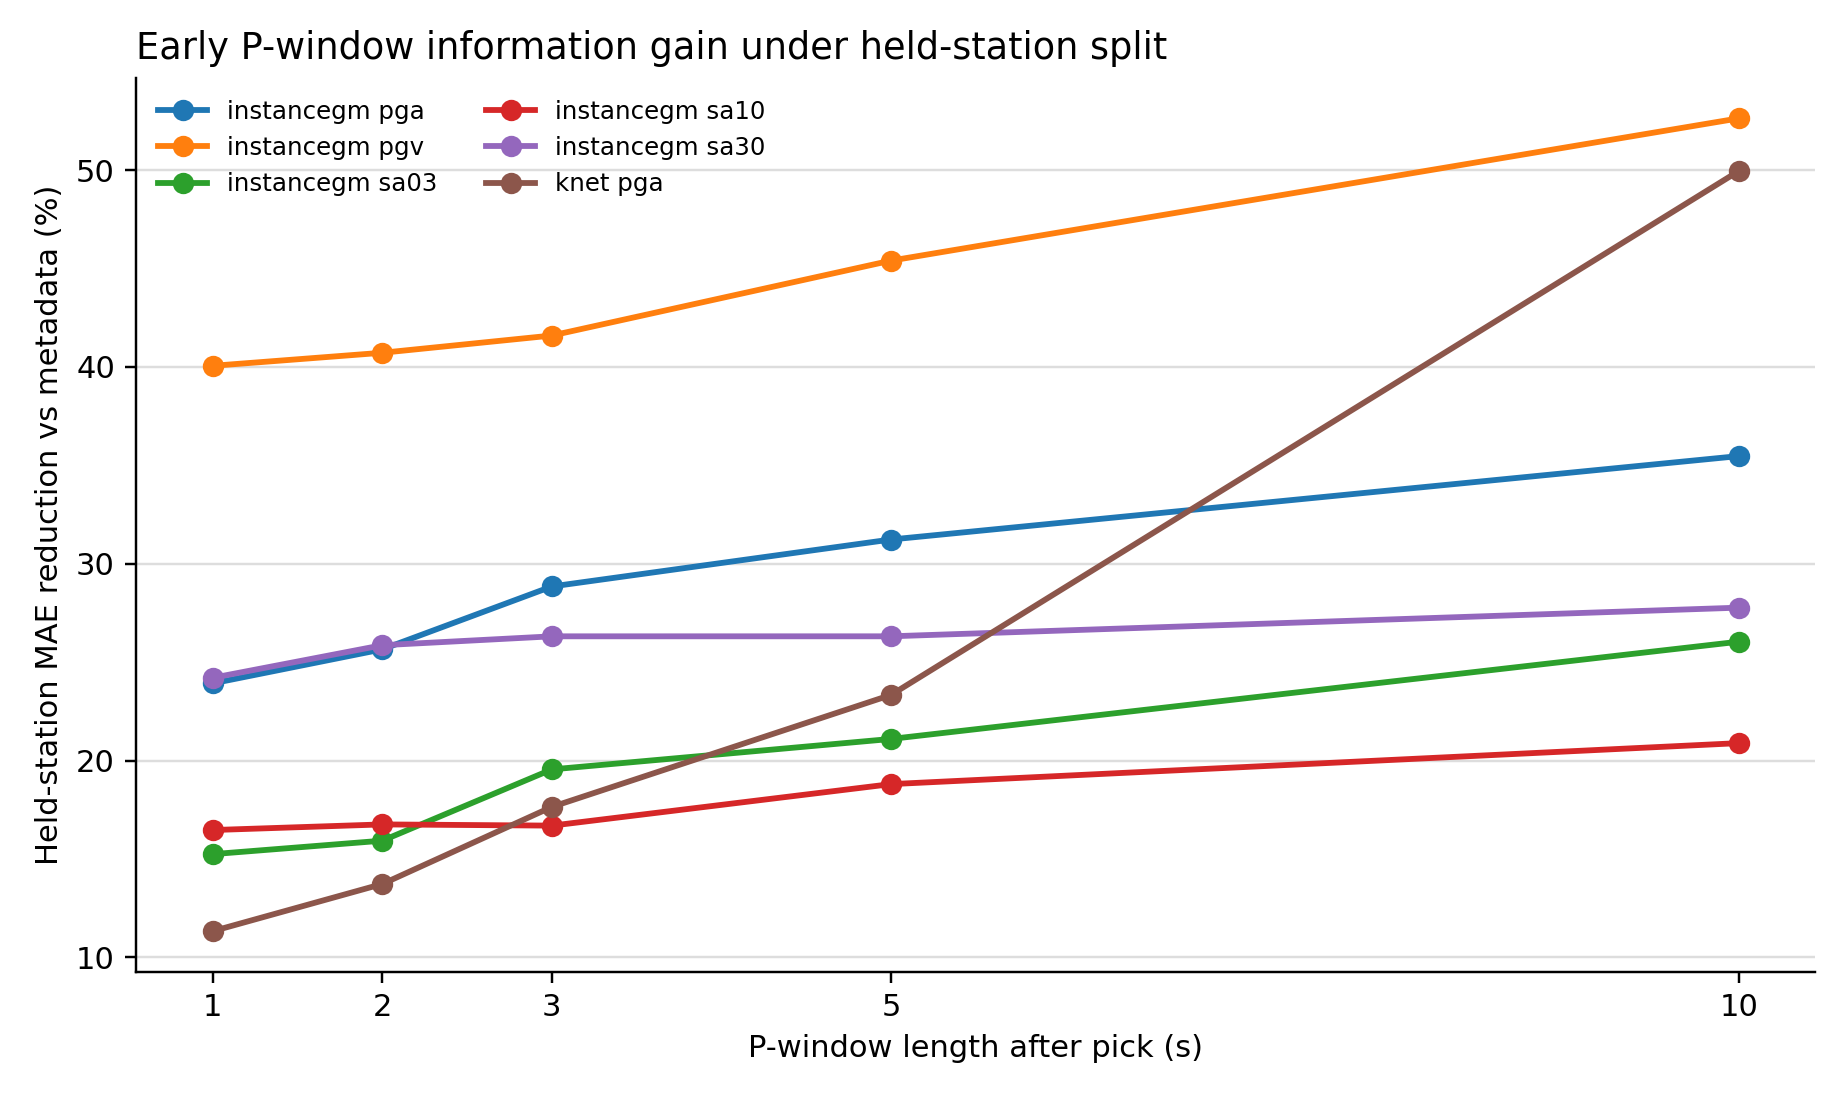
\includegraphics[keepaspectratio,alt={P 窗口长度控制早期地震动信息增益。误差降低率随窗口增长增强，但不同目标的增长速率不同。 Fig. 2 P-window length controls the information gain for strong-motion prediction.}]{figures/ground_motion_audit/held_station_window_scan.png}}
\caption{P
窗口长度控制早期地震动信息增益。误差降低率随窗口增长增强，但不同目标的增长速率不同。
Fig. 2 P-window length controls the information gain for strong-motion
prediction.}
\end{figure}

\subsubsection{2.2
增益通过重采样、支持域和尾部检验}\label{ux589eux76caux901aux8fc7ux91cdux91c7ux6837ux652fux6301ux57dfux548cux5c3eux90e8ux68c0ux9a8c}

paired bootstrap 显示，六个主目标的 95\% 置信区间下界均为正。最弱下界为
InstanceGM SA10 的 16.9\%；K-NET PGA 的平均降低率为 49.9\%，置信区间为
46.6\%--53.1\%。该结果说明增益在测试记录重采样下保持稳定。

source-path support 审计保留 82.4\%--83.9\% 的 held-station
测试记录。该审计只使用震级和距离筛选，不用目标幅值。筛选后六个主目标仍均为正增益，范围为
20.1\%--54.5\%。这降低了``测试样本落在训练集支持域外导致表观增益''的解释空间。

强震动尾部结果更接近预警风险。目标幅值最高 5\%
的记录中，早期波形对所有主目标的尾部 MAE 均有降低，范围为
18.9\%--66.0\%。同时，factor-2 underprediction 没有完全消失，InstanceGM
SA30 的最强尾部还出现轻微恶化。该结果限定了本文结论：早期 P
波能减少强震动尾部误差，仍不能消除高后果漏报边界。

\begin{figure}
\centering
\pandocbounded{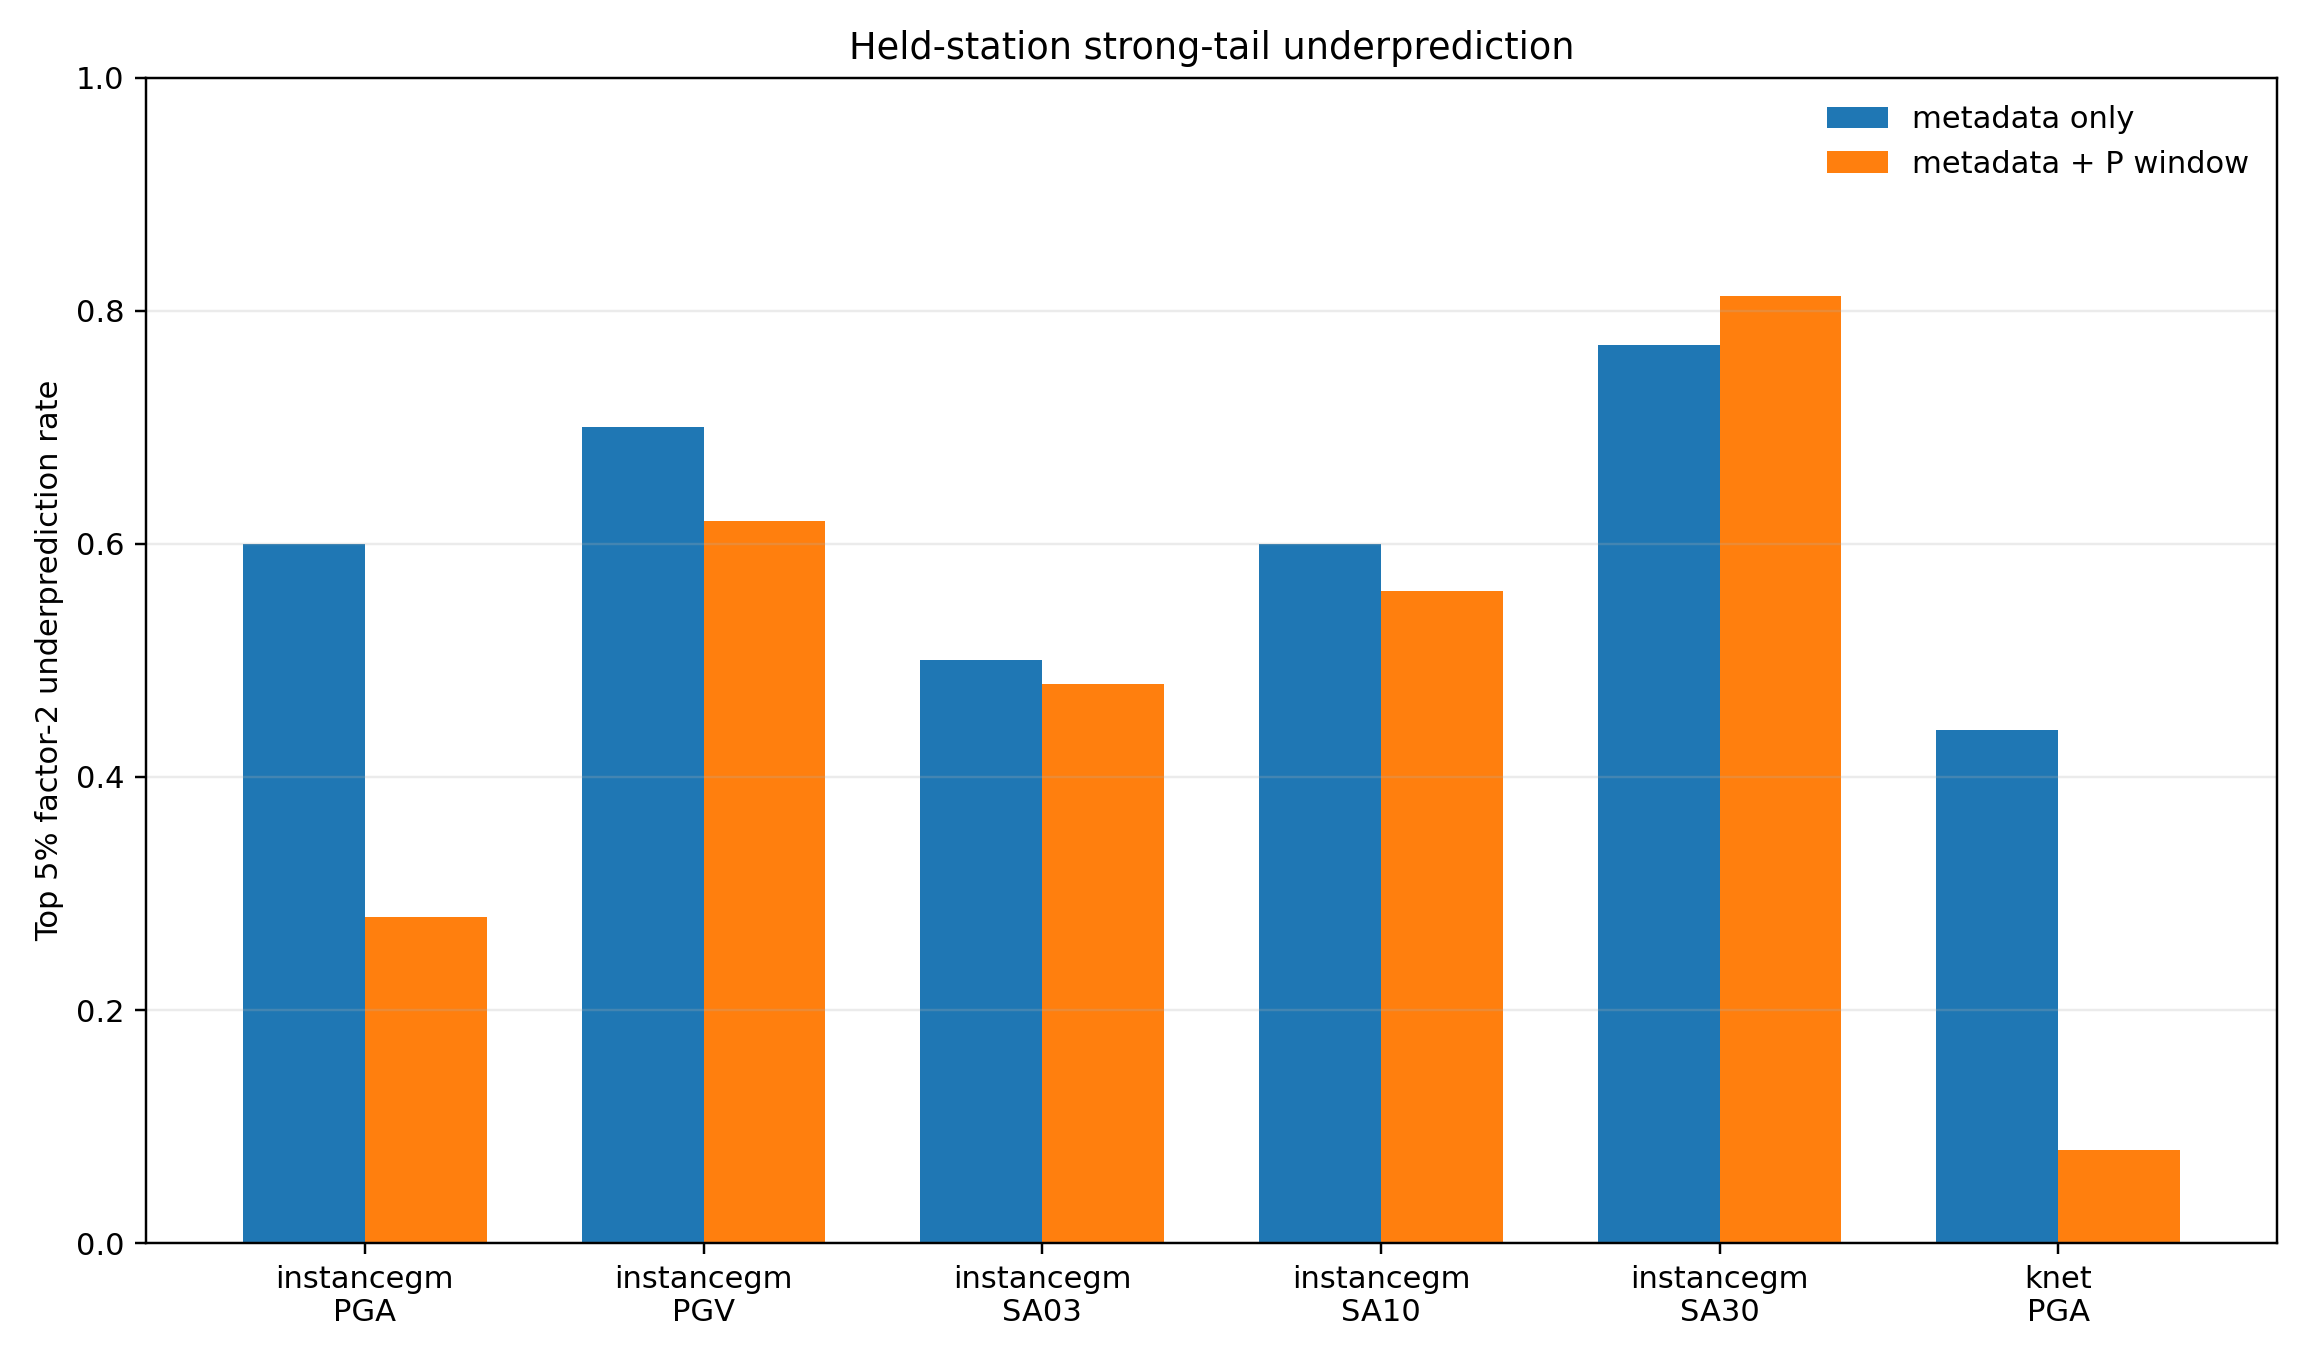
\includegraphics[keepaspectratio,alt={稳健性和尾部审计。Bootstrap、support 限制和强震动尾部检验均保留正增益，同时显示残余漏报风险。 Fig. 3 Robustness and tail audits retain positive gains and expose residual miss risk.}]{figures/ground_motion_audit/held_station_tail_audit.png}}
\caption{稳健性和尾部审计。Bootstrap、support
限制和强震动尾部检验均保留正增益，同时显示残余漏报风险。 Fig. 3
Robustness and tail audits retain positive gains and expose residual
miss risk.}
\end{figure}

\subsubsection{2.3 pre-peak 审计给出短窗 lead-time
边界}\label{pre-peak-ux5ba1ux8ba1ux7ed9ux51faux77edux7a97-lead-time-ux8fb9ux754c}

短 P 窗口可能已经包含接近最终 PGA
的峰值。若不加区分，模型可能利用已经出现的强震动峰值，削弱预警前瞻性解释。K-NET
pre-peak 审计筛选 early horizontal peak 低于最终 PGA 80\%
的记录。在这个子集中，1 s 和 3 s 窗口仍分别降低 MAE 13.8\% 和
17.9\%。这一结果支撑 1--3 s 短窗的 lead-time 信息增益。10 s
窗口结果更适合解释为 early strong-motion
information，部分记录在该时间尺度下已接近后续强震动阶段。

\subsubsection{2.4
外部公开数据层保留同一信息增益}\label{ux5916ux90e8ux516cux5f00ux6570ux636eux5c42ux4fddux7559ux540cux4e00ux4fe1ux606fux589eux76ca}

AQ2009GM 作为独立 SeisBench
强震动数据层，提供了更大规模的外部检验。全部本地 manifest chunk
被流式处理后，原始 chunk 文件被删除，只保留特征表和 inventory。5 s
held-station 测试中，AQ2009GM PGA 和 PGV 的误差降低率分别为 55.8\% 和
71.9\%。该结果说明早窗信息增益并不局限于 InstanceGM 和 K-NET。

CWA 提供官方 PGA/PGV metadata target。当前结果只覆盖公开 benchmark 的
2011 年，不代表完整 CWA 2011--2021 年验证。held-station 测试中，2 s 窗口
PGA/PGV 的 MAE 分别降低 14.6\% 和 17.7\%，5 s 窗口分别降低 29.9\% 和
40.3\%。该层样本量小于
AQ2009GM，目标变量来自官方数据表，是重要独立证据。

ESM 外部域使用欧洲强震动记录。本地头段缺少显式 P 到时，本文使用理论 P
到时，并通过 Vp 敏感性和 envelope onset spot audit 检查对齐误差。Vp=5.5
km/s 相对 6.0 km/s 的中位延迟为 2.517 s，Vp=6.5 km/s 的中位提前为 2.130
s。200 条波形 envelope onset spot audit 中，86
条高置信记录的中位绝对偏移为 1.223 s，95 分位为 3.960 s。ESM
结果用于外部强震动和 transfer 检验，不写成 catalog/manual P-pick 证据。

\begin{figure}
\centering
\pandocbounded{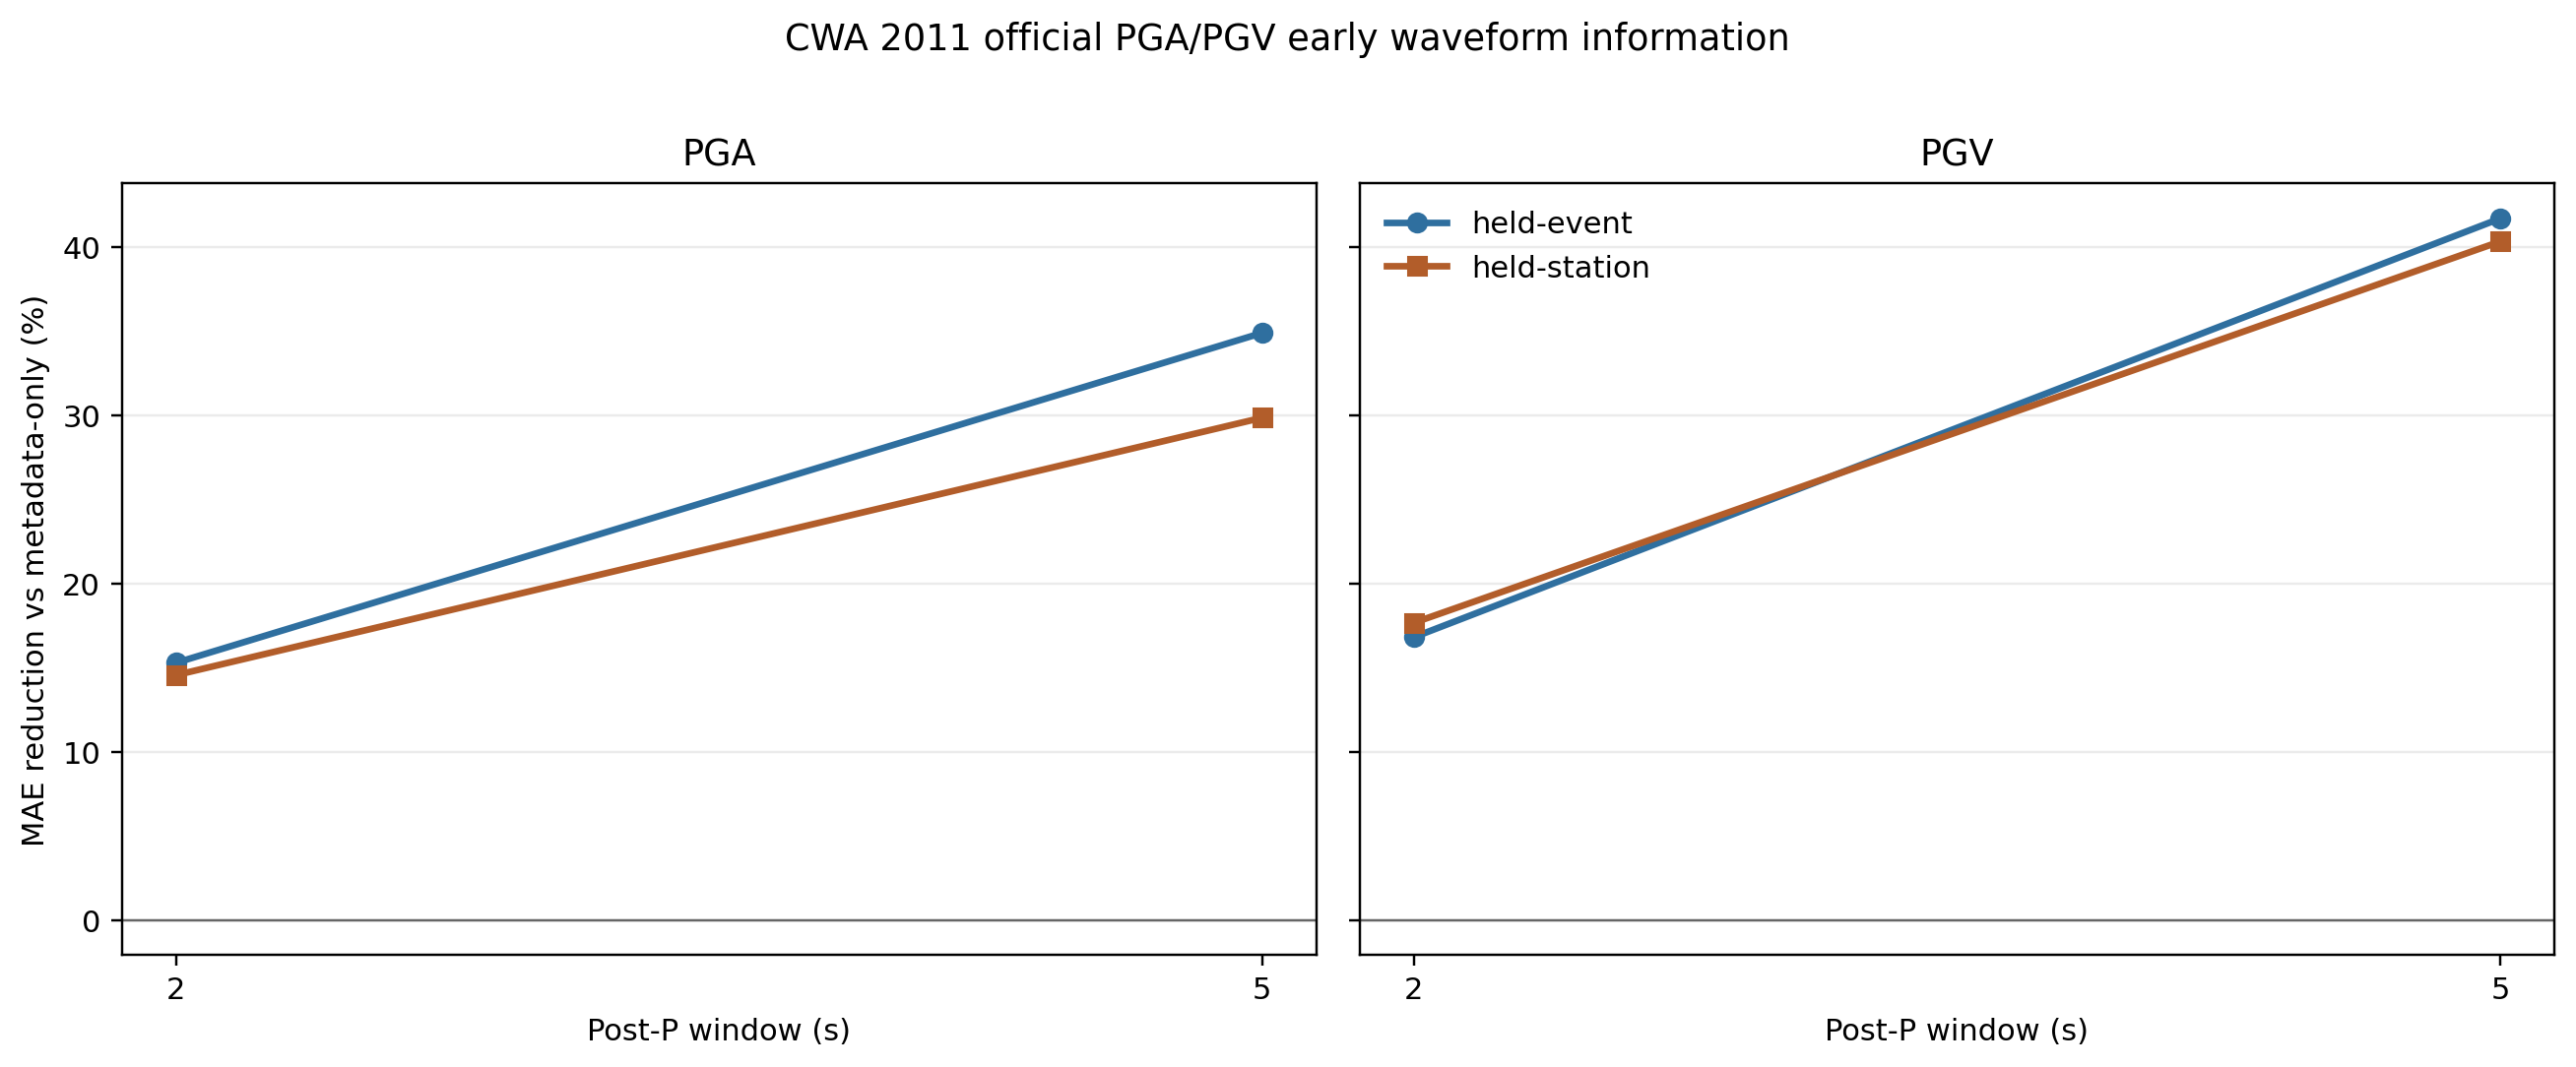
\includegraphics[keepaspectratio,alt={外部公开数据层。AQ2009GM、CWA 和 ESM 从不同数据来源支持同一早窗信息增益，同时各自带有明确的数据边界。 Fig. 4 External public-data layers support the same early-window information gain with explicit data boundaries.}]{figures/ground_motion_audit/cwa_official_pga_pgv_panel.png}}
\caption{外部公开数据层。AQ2009GM、CWA 和 ESM
从不同数据来源支持同一早窗信息增益，同时各自带有明确的数据边界。 Fig. 4
External public-data layers support the same early-window information
gain with explicit data boundaries.}
\end{figure}

\subsubsection{2.5 经典参考和区域 GMM screening 支持 added-information
结论}\label{ux7ecfux5178ux53c2ux8003ux548cux533aux57df-gmm-screening-ux652fux6301-added-information-ux7ed3ux8bba}

本文使用低参数 attenuation-shaped ridge、bias-corrected OpenQuake
BooreEtAl2014、K-NET 日本 GMM screening 和 ESM regional GMM screening
作为经典参考。InstanceGM 当前 split 中有 Vs30；K-NET 缺少 Vs30、rupture
distance 和 focal mechanism，K-NET GMM 结果保持 screening reference
定位。

在相同 held-station 行上，metadata 加早期波形模型优于 BooreEtAl2014
参考。相对 BooreEtAl2014，InstanceGM PGA、PGV、SA03、SA10、SA30 和 K-NET
PGA 的 MAE 分别降低 36.6\%、59.4\%、35.4\%、36.4\%、48.0\% 和
60.6\%。K-NET PGA 的日本 GMM screening 中，最佳候选 Kanno2006Shallow 的
MAE 为 0.242，早期波形模型为 0.111。

ESM regional GMM screening 使用
BooreEtAl2014、AkkarEtAl2014、BindiEtAl2014 和 CauzziEtAl2015
候选。相对最佳 screened regional GMM，早期 P+distance+site 模型在 2 s
PGA/PGV 上降低 MAE 34.8\%/23.8\%，5 s 为 48.3\%/30.2\%，10 s 为
43.1\%/30.4\%。这个层增强了经典参考对照，但仍是 screening，因为 rupture
geometry、rake 和完整构造类型信息不完备。

\begin{figure}
\centering
\pandocbounded{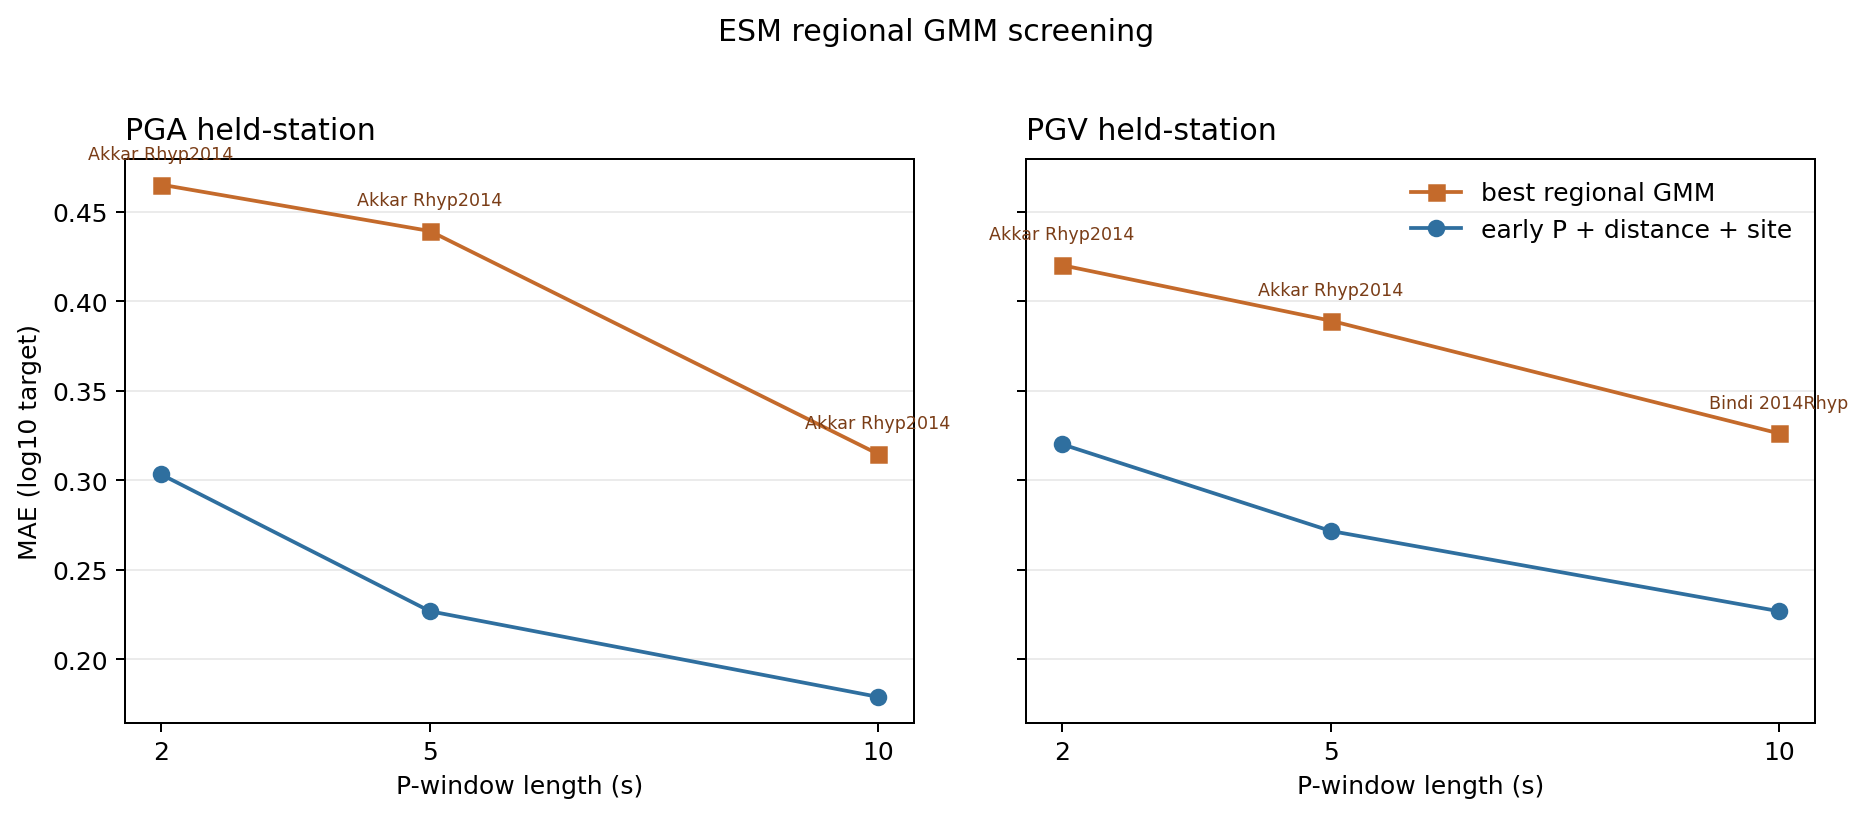
\includegraphics[keepaspectratio,alt={经典参考和 GMM screening。早期 P 波信息在相同测试行上超过可用经典参考，但部分 GMM 输入缺失使该层保持 screening 定位。 Fig. 5 Classical references and GMM screening support the added-information result.}]{figures/ground_motion_audit/esm_regional_gmm_screening.png}}
\caption{经典参考和 GMM screening。早期 P
波信息在相同测试行上超过可用经典参考，但部分 GMM 输入缺失使该层保持
screening 定位。 Fig. 5 Classical references and GMM screening support
the added-information result.}
\end{figure}

\subsubsection{2.6 跨区域 transfer
揭示可预测性边界}\label{ux8de8ux533aux57df-transfer-ux63edux793aux53efux9884ux6d4bux6027ux8fb9ux754c}

跨区域 direct transfer
的结果显示，源区域模型不能直接等同于目标区域模型。四域 transfer
只使用早期波形统计，不使用震级、距离、场地、event id 或 station id。2 s
窗口下，source-only transfer 的 MAE penalty 中位数为 2.94 倍；5 s
窗口升至 4.30 倍。target-offset calibration 能把 penalty 降至 1.56 倍和
1.84 倍，但仍高于目标域训练。

不确定性边界更加明显。source-domain conformal interval
在跨区应用时欠覆盖，2 s 和 5 s 的覆盖率中位数分别为 0.468 和
0.298，远低于 0.90 标称覆盖率。目标区 offset 和 conformal
残差宽度校准后，50 条目标区校准记录已使覆盖率中位数接近 0.90，100
条记录更稳定。代价是区间宽度显著增大，2 s 和 5 s 在 100
条校准记录时的中位区间宽度分别为 2.161 和 2.080 log10 units。

该结果给出了本文最重要的边界：早期 P
波在目标域内具有可测量信息增益；源域残差分布不能直接代表目标域不确定性；少量目标域样本可以修复覆盖率，但不能消除跨区域地震动差异。

\begin{figure}
\centering
\pandocbounded{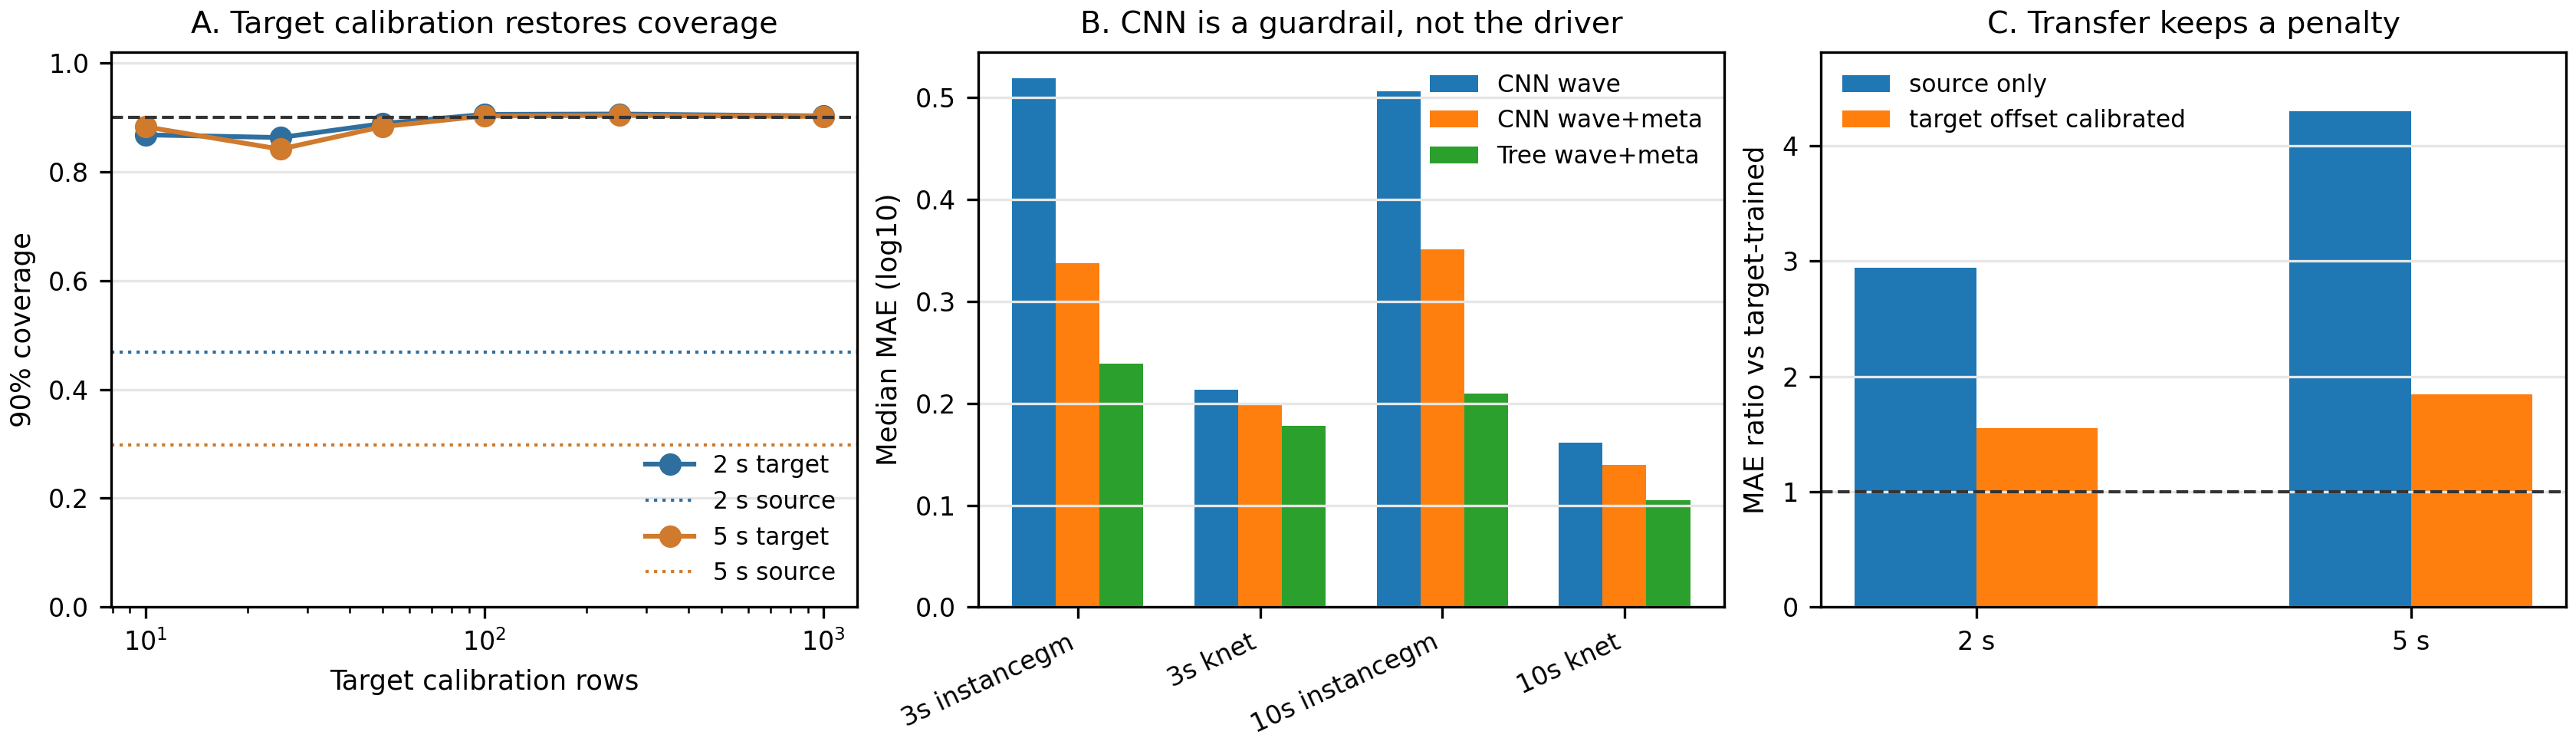
\includegraphics[keepaspectratio,alt={跨区域可预测性边界。更多早期波形信息提高域内预测能力，同时跨区域 direct transfer 保留明显 penalty；目标区校准可恢复覆盖率但扩大区间。 Fig. 6 Cross-region predictability boundary.}]{figures/ground_motion_audit/nc_supplementary_experiments_summary.png}}
\caption{跨区域可预测性边界。更多早期波形信息提高域内预测能力，同时跨区域
direct transfer 保留明显 penalty；目标区校准可恢复覆盖率但扩大区间。
Fig. 6 Cross-region predictability boundary.}
\end{figure}

\subsubsection{2.7 轻量 CNN
对照限定模型复杂度解释}\label{ux8f7bux91cf-cnn-ux5bf9ux7167ux9650ux5b9aux6a21ux578bux590dux6742ux5ea6ux89e3ux91ca}

本文补充了一个小型 CNN
波形编码器对照。该模型直接读取早期波形窗口，并分别测试 waveform-only 和
waveform+metadata 设置。结果显示，小 CNN 能学习到强震动信息；K-NET PGA
10 s waveform+metadata 的 MAE 为 0.139，\(R^2\) 为
0.799。在当前样本量和训练设置下，稳定树模型和手工早窗统计仍取得更低误差。InstanceGM
10 s 中位 MAE：CNN waveform-only 为 0.506，CNN waveform+metadata 为
0.351，树模型 waveform+metadata 为 0.210；K-NET 10 s PGA 分别为
0.161、0.139 和 0.105。

这个对照的作用是限定模型解释。本文不依赖复杂神经网络获得主结论，也不把
CNN 结果写成最优模型。主证据来自公开数据、严格
split、强震动尾部审计、跨区域 transfer 和 conformal 不确定性边界。

\subsection{3 讨论}\label{ux8ba8ux8bba}

本文结果说明，早期 P 波预测强震动的可用信息是可以用公开数据量化的。域内
held-station 测试、强震动尾部审计和多个外部数据层给出一致方向：P
到时后的短窗口确实包含 metadata
之外的信息。该结论的地震学意义在于，早期台站观测不仅是快速震级估计的替代输入，也携带了目标台站路径和局部响应的综合观测约束。

边界同样清楚。强震动尾部仍存在 factor-2
underprediction；部分大残差在不同目标中重复出现；K-NET PGA
大残差偏向更远距离；跨区域 source conformal
区间严重欠覆盖。这些现象说明，早期 P
波可以降低误差，强震动预测仍然需要显式不确定性。对于预警系统，高风险尾部和跨区域校准应进入模型输出设计。

目标区校准样本量结果对实际部署有直接启发。50--100 条目标区记录已经能将
conformal
覆盖率拉回接近标称水平。这个数量并不大，说明新区域部署时，可以通过少量本地强震动记录修正偏差和区间宽度。区间仍然很宽，反映的是物理和数据分布差异，而非校准失败。

本文也有明确限制。CWA 结果目前只覆盖 2011 年公开 benchmark；ESM P
到时来自理论到时而非人工拾取；K-NET GMM 对照缺少完整 Vs30、rupture
distance 和 focal mechanism；AQ2009GM 保留的是特征表而非原始
chunk。上述限制不影响``公开数据下早窗信息增益存在''的主结论，但限制了每个外部层可支持的强度。

后续工作应集中在三方面。第一，增加带人工或官方 P 到时的小样本 ESM
验证，直接检验理论 P 到时带来的窗口误差。第二，在更多区域建立完整 GMM
输入，用区域化 GMM 对照替代
screening。第三，把本文离线边界嵌入实时预警流程，评估通信延迟、报警阈值和用户代价下的可用性。

\subsection{4 结论}\label{ux7ed3ux8bba}

（1）公开强震动数据可以构建事件-台站级早期 P
波预测基准。统一清单、分量和单位 provenance、held-event/held-station
split 以及外部数据层共同限制了证据边界。

（2）早期 P 波在未见台站测试中提供 metadata 之外的信息。10 s 窗口下
InstanceGM PGA、InstanceGM PGV 和 K-NET PGA 的 MAE 分别降低
35.5\%、52.6\% 和 49.9\%；短窗 pre-peak 子集仍保留正增益。

（3）强震动尾部和外部数据层支持同一方向。AQ2009GM、CWA 2011 年官方
PGA/PGV 层和 ESM screening
均显示早窗信息增益，同时暴露了各自的数据限制。

（4）跨区域 transfer 的主要结论是可预测性边界。source conformal interval
在目标区欠覆盖，少量目标区校准样本可恢复覆盖率，区间宽度同步增大，说明区域不确定性需要显式建模。

（5）轻量 CNN
对照显示，主结论不依赖复杂模型。稳定树模型和透明特征更适合作为当前基准的主分析工具。

\subsection{数据和代码可用性}\label{ux6570ux636eux548cux4ee3ux7801ux53efux7528ux6027}

本文使用的公开数据来自各数据提供方。派生特征表、split、metrics、图件和验证报告保存在本地仓库输出目录；原始受限或体量过大的波形文件不随稿件重新分发。AQ2009GM
和 CWA 原始临时文件在特征提取后已删除，仅保留复现实验所需的小特征表和
inventory。最终公开仓库需要删除本地路径、缓存记录和不应公开的数据副本。

\subsection{利益冲突声明}\label{ux5229ux76caux51b2ux7a81ux58f0ux660e}

作者声明无利益冲突。

\subsection{参考文献初稿说明}\label{ux53c2ux8003ux6587ux732eux521dux7a3fux8bf4ux660e}

参考文献条目将在终稿前按目标期刊格式逐条核对。当前正文需要覆盖地震预警基本文献、PhaseNet/EQTransformer
相位拾取文献、InstanceGM/K-NET/ESM/CWA/AQ2009GM
数据源文献、BooreEtAl2014、AkkarEtAl2014、BindiEtAl2014、CauzziEtAl2015
和 Kanno2006 等 GMM 文献，以及 conformal prediction 和区域迁移评估文献。

\end{document}
